\documentclass[12pt,a4paper]{article}
\usepackage[utf8]{inputenc}
\usepackage[french]{babel}
\usepackage[T1]{fontenc}
\usepackage{amsmath}
\usepackage{amsfonts}
\usepackage{amssymb}
\usepackage{makeidx}
\usepackage{lmodern}
\usepackage{authblk}
\usepackage[skip=10pt plus1pt, indent=20pt]{parskip}
\usepackage{enumitem}
\usepackage{pdfpages}
\usepackage{fancyhdr}
\usepackage{geometry}
\usepackage{xparse}
\usepackage{float}

%%%% debugging de l'affichage : à commenter pour cacher les frames %%%%

%\usepackage[]{showframe}

%%%% authblk en fr %%%%

\renewcommand\Authand{, }
\renewcommand\Authands{ et }


\floatstyle{ruled}
\restylefloat{figure}


\setlength{\textheight}{1.15\textheight}
\setlength{\headheight}{15.35403pt}


\makeatletter
\NewDocumentCommand\headerspdf{ O {pages=-} m }{% [options for include pdf]{filename.pdf}
  \includepdf[%
    #1,
    pagecommand={\thispagestyle{fancy}},
    scale=.7,
    ]{#2}}
\NewDocumentCommand\secpdf{somO{1}m}{% [short title]{section title}[page specification]{filename.pdf} --- possibly starred
  \clearpage
  \thispagestyle{fancy}%
  \includepdf[%
    pages=#4,
    pagecommand={%
      \IfBooleanTF{#1}{%
        \section*{#3}}{%
        \IfNoValueTF{#2}{%
          \section{#3}}{%
          \section[#2]{#3}}}},
    scale=.65,
    ]%
    {#5}}
\makeatother

\pagestyle{fancy}

\author{Valentin \bsc{RIEU-FERRARA}}
\author{Mourtaza \bsc{AKIL}}
\author{Hany \bsc{BAYAZID}}
\author{Bruno \bsc{ROMAIN}}
\affil{Université Jean Monnet}
\date{\today}
\title{Cahier des charges}
\begin{document}

\maketitle

\newpage
\tableofcontents

\newpage

\section{Descriptif}

	Notre projet consistera à réaliser une plateforme d'édition collaborative de documents textes riches (style word, google docs). Notre plateforme ressemblera typiquement à ce que propose Microsoft Word, mais avec moins de fonctionnalités.

\section{Fonctionnalités}

	\subsection{Principales}
	Voici une liste des fonctionnalités qu'on implémentera initialement : \par
	
	\begin{itemize}
		\item \textbf{Création de documents} : \par Un utilisateur pourra utiliser la plateforme pour créer un nouveau document et indiquer les caractéristiques de celui-ci. Pour une première version, il n'y aura pas un large éventail de choix. Mais pour la version finale, il aura la possiblité de choisir parmi ces fonctionnalités et éventuellement d'autres (qu'on pense implémenter) : \par 
		\begin{itemize}
			\item[$\bullet$] Choix sur la police,
			\item[$\bullet$] Génération de structures déjà faites,
			\item[$\bullet$] Table des matières dynamique.
		\end{itemize}
		
		\item \textbf{Téléchargement} : \par Tout document, du moment qu'il puisse l'être, pourra être téléchargé au format PDF (au moins). On tentera également d'implémenter la possibilité de le télécharger au format utilisé par la plateforme.
		
		\item \textbf{Organisation de sessions de travail autour d'un document} : \par Un utilisateur pourra décider de mettre en partage ses documents, c'est-à-dire l'option d'organiser des sessions de collaboration auxquelles d'autres utilisateurs pourront demander l'accès (par un lien par exemple) pour qu'ils puissent lire/modifier un document simultanément.
		
		\item \textbf{Système de status} : \par Tous les utilisateurs connectés auront un ensemble de statuts et en fonction de ces statuts, ils auront l'accés à certaines options et services. Tous les utilisateurs connectés à la session seront par exemple considérés comme des \emph{collaborateurs}
		
		\item \textbf{Options} : \par 
		Les collaborateurs auront l'accés à une panoplie d'options en fonction de leur statuts. Par exemple, tout \emph{collaborateur} (collaborateur étant un statut) aura au moins la possibilité de lire en temps réel le document et un accès permanent à la messagerie de la session.
		
		\item \textbf{Messagerie} : \par 
		Un utilisateur connecté pourra envoyer des messages à tout autre utilisateur lorsqu'ils sont, soit connectés à une même session de travail, soit membres de la même équipe de travail. 
		
	\end{itemize}
	
	\newpage
	\subsection{Secondaires}
	
		Voici certaines des fonctionnalités de travail qu'on ajoutera aux fonctionnalités principales : \par 
		
		\begin{itemize}
		
			\item \textbf{Mise en place d'équipes de travail} : \par
			Un utilisateur pourra créer une équipe de travail dans laquelle il accordera des statuts aux membres de l'équipe. La différence avec les sessions de travail se trouvent dans l'idée qu'une équipe de travail est permanente alors qu'une session de travail aura une durée de vie. De plus, dans une équipe, dans une äuipe de travail, il y aura également un système de hiérarchie plus complexe que celui des sessions de travail. \par
			Les membres d'une équipe auront accès à tous les documents réalisés dans le cadre du "projet" pour lequel l'équipe existe.
			
			\item \textbf{Commentaires} : \par
			L'idée d'intégrer les commentaires et annotations nous semble intéressante. Ce sera probablement l'une des fonctionnalités qu'on tentera d'intégrer parmi les secondaires.
			
			
			\item \textbf{Liens/références dynamiques} : \par
			On pense également à implémenter un système de liens dynamiques qui permettra de référencer une section du document dans un message.
		
			
		\end{itemize}
		
		\section{Architecture}
		
		En terme d'architecture, on reprendra exactement ce qui est demandé dans le sujet :
		
		\begin{itemize}
		
			\item Un serveur qui hébergera les documents, qui servira d'intermédiaire de communication entre les clients que ce soit pour la messagerie ou l'écriture collaborative de documents. Il stockera également toutes les informations sur les utilisateurs, équipes, sessions de travail.
			
			\item Le client léger/lourd permettra de se connecter, ou non (pour la réalisation de documents à court terme), et ensuite de travailler sur des documents personnels ou des documents collaboratifs (uniquement si identifié) : \par
			
			\begin{itemize}
			
				\item[$\bullet$] Le client léger, qui aura plus ou moins les mêmes options que le client lourd, en ligne via une connexion Web.
				
				\item[$\bullet$] Le client lourd, qui permettra une connexion via une application en \textsl{Swing/JavaFX}.
			\end{itemize}
		\end{itemize}
		
		Au niveau de l'organisation du projet, on aura un projet java qui implémentera le client lourd et un projet web dynamique, qui servira de serveur de données (communication avec la base de données, intermédiaire entre les clients, etc) et serveur web pour la plateforme web. 
		
	\section{Plan de la plateforme}

	Voici, globalement, les étapes à réaliser pour utiliser notre plateforme :
	
	\begin{itemize}
	
		\item L'utilisateur, en arrivant sur la plateforme, devra avant tout s'authentifier. Une interface de connexion sera donc mise en place, aussi bien côté swing que côté web.
		
		\item Il accèdera ensuite à un panneau qui lui permettra soit de charger des documents sur lesquels il a déjà travaillé, soit d'en créer un nouveau.
		
		\item S'il a demandé à créer un nouveau, un panneau de mise en forme pré-traitement lui sera ouvert.
		
		\item Il aura ensuite accès au panneau d'édition sur lequel il aura 3 sections (pour l'instant) : \par
		
		\begin{itemize}
			
			\item[$\bullet$] Une barre de menu qui va lui permettre des options sur le fichier (sauvegarde, chargement, exportation, annuler modification, etc)
			
			\item[$\bullet$] Un panneau qui donner accès à tous les outils de gestion de mise en forme, police, listes, couleurs, etc.
			
			\item[$\bullet$] Le panneau d'édition de texte.
		
		\end{itemize}
	
	\end{itemize}
	
	\section{Base de données}
	
	Pour l'instant, notre base de données est plutôt élémentaire. Elle n'a que deux tables. En fonction des fonctionnalités qu'on implémentera, on suppose que cette base s'enrichira.
	
	\begin{itemize}
		
		\item Une table qui va stocker les informations sur les utilisateurs : \par
		
		\begin{itemize}
			
			\item[$\bullet$] Un identifiant unique
			
			\item[$\bullet$] Un mot de passe crypté
			
			\item[$\bullet$] La liste des documents auxquels il a accès
			
		\end{itemize}
		
		\item Une table qui va stocker les informations sur les documents : \par
		
		\begin{itemize}
		
			\item[$\bullet$] Un identifiant unique
			
			\item[$\bullet$] Le nom du fichier
			
			\item[$\bullet$] Caractéristiques (format, taille, etc)
			
			\item[$\bullet$] Propriétaire
			
			\item[$\bullet$] Liste des collaborateurs (personnes qui y ont accès en plus du propriétaire)
			
			\item[$\bullet$] Date de dernière modification
		
		\end{itemize}
	
	\end{itemize}
	
	\newpage
	
	\section{Répartition du travail - Organisation de l'équipe - Technologies utilisées}
	
	Notre projet sera divisé en 3 grosses sections : \par
	
	\begin{itemize}

		\item Le client lourd sera programmé en Swing, comme demandé dans le sujet. Cette partie sera essentiellement gérée et effectuée par \textbf{Mourtaza AKIL}.
		
		\item Le client léger sera implémenté par \textbf{Valentin RIEU}. Il utilisera essentiellement les technologies vues en cours et Développement Web I, l'année dernière. Des frameworks tels que JQuery et Bootstrap pourront éventuellement être utilisés.
		
		\item Le serveur de données sera géré par \textbf{Bruno ROMAIN} et \textbf{Hany BAYAZID} et utilisera notamment la communication TCP pour le client lourd et une communication via les servlets pour le client léger. Il puisera ses ressources (informations, fichiers, etc) dans une base de données.
	
	\end{itemize}
	
	Notre chef de projet sera : \textbf{Mourtaza AKIL}.
	
	\section{Annexes}
	\appendix
	
	\subsection{Diagramme de cas d'utilisation}

	\begin{figure}[hb]
		\centering

		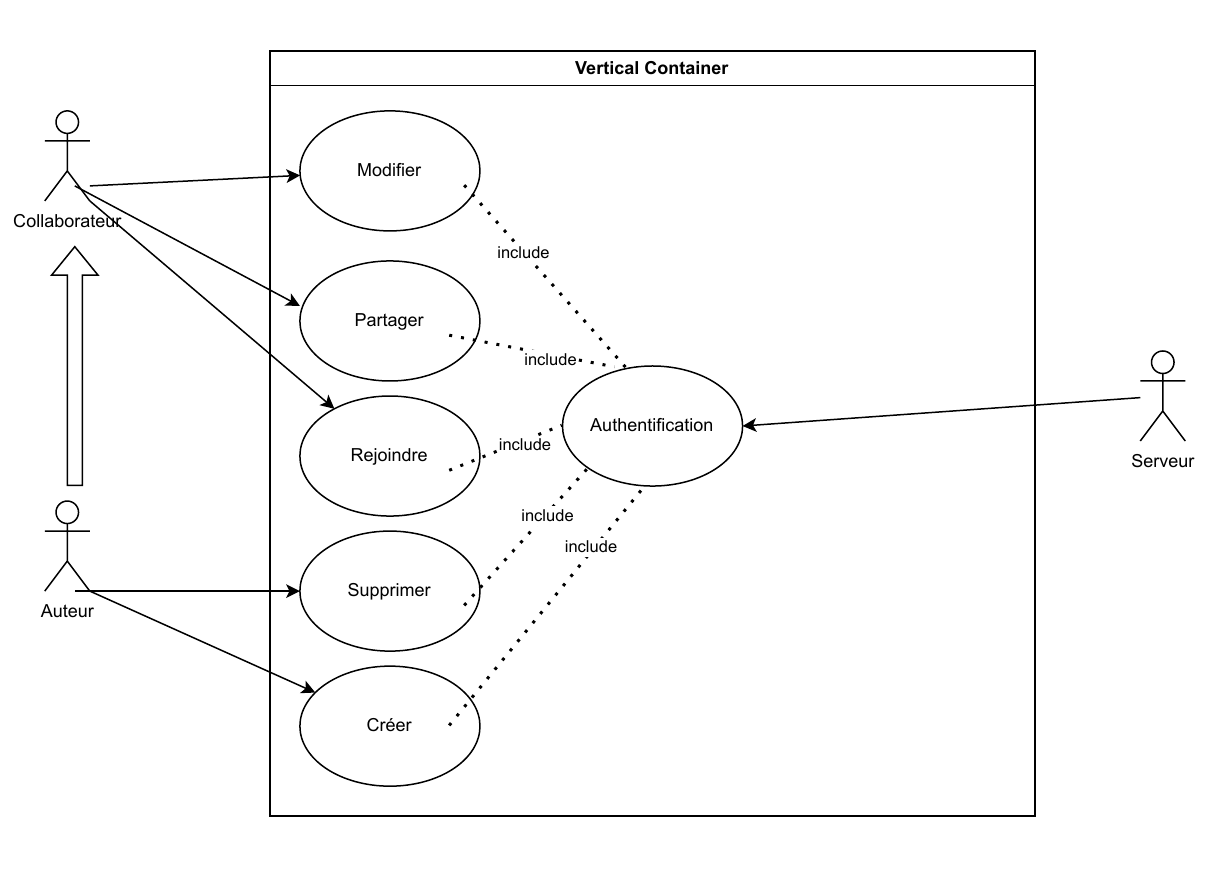
\includegraphics[scale=.3]{setup/diagramme_de_cas.png}
	\caption{Diagramme de cas d'utilisation}	
	\end{figure}
	\newpage
	
	\subsection{Diagramme de séquence de partage}
	
	\begin{figure}[hb]
		\vspace*{1em}
		\centering
		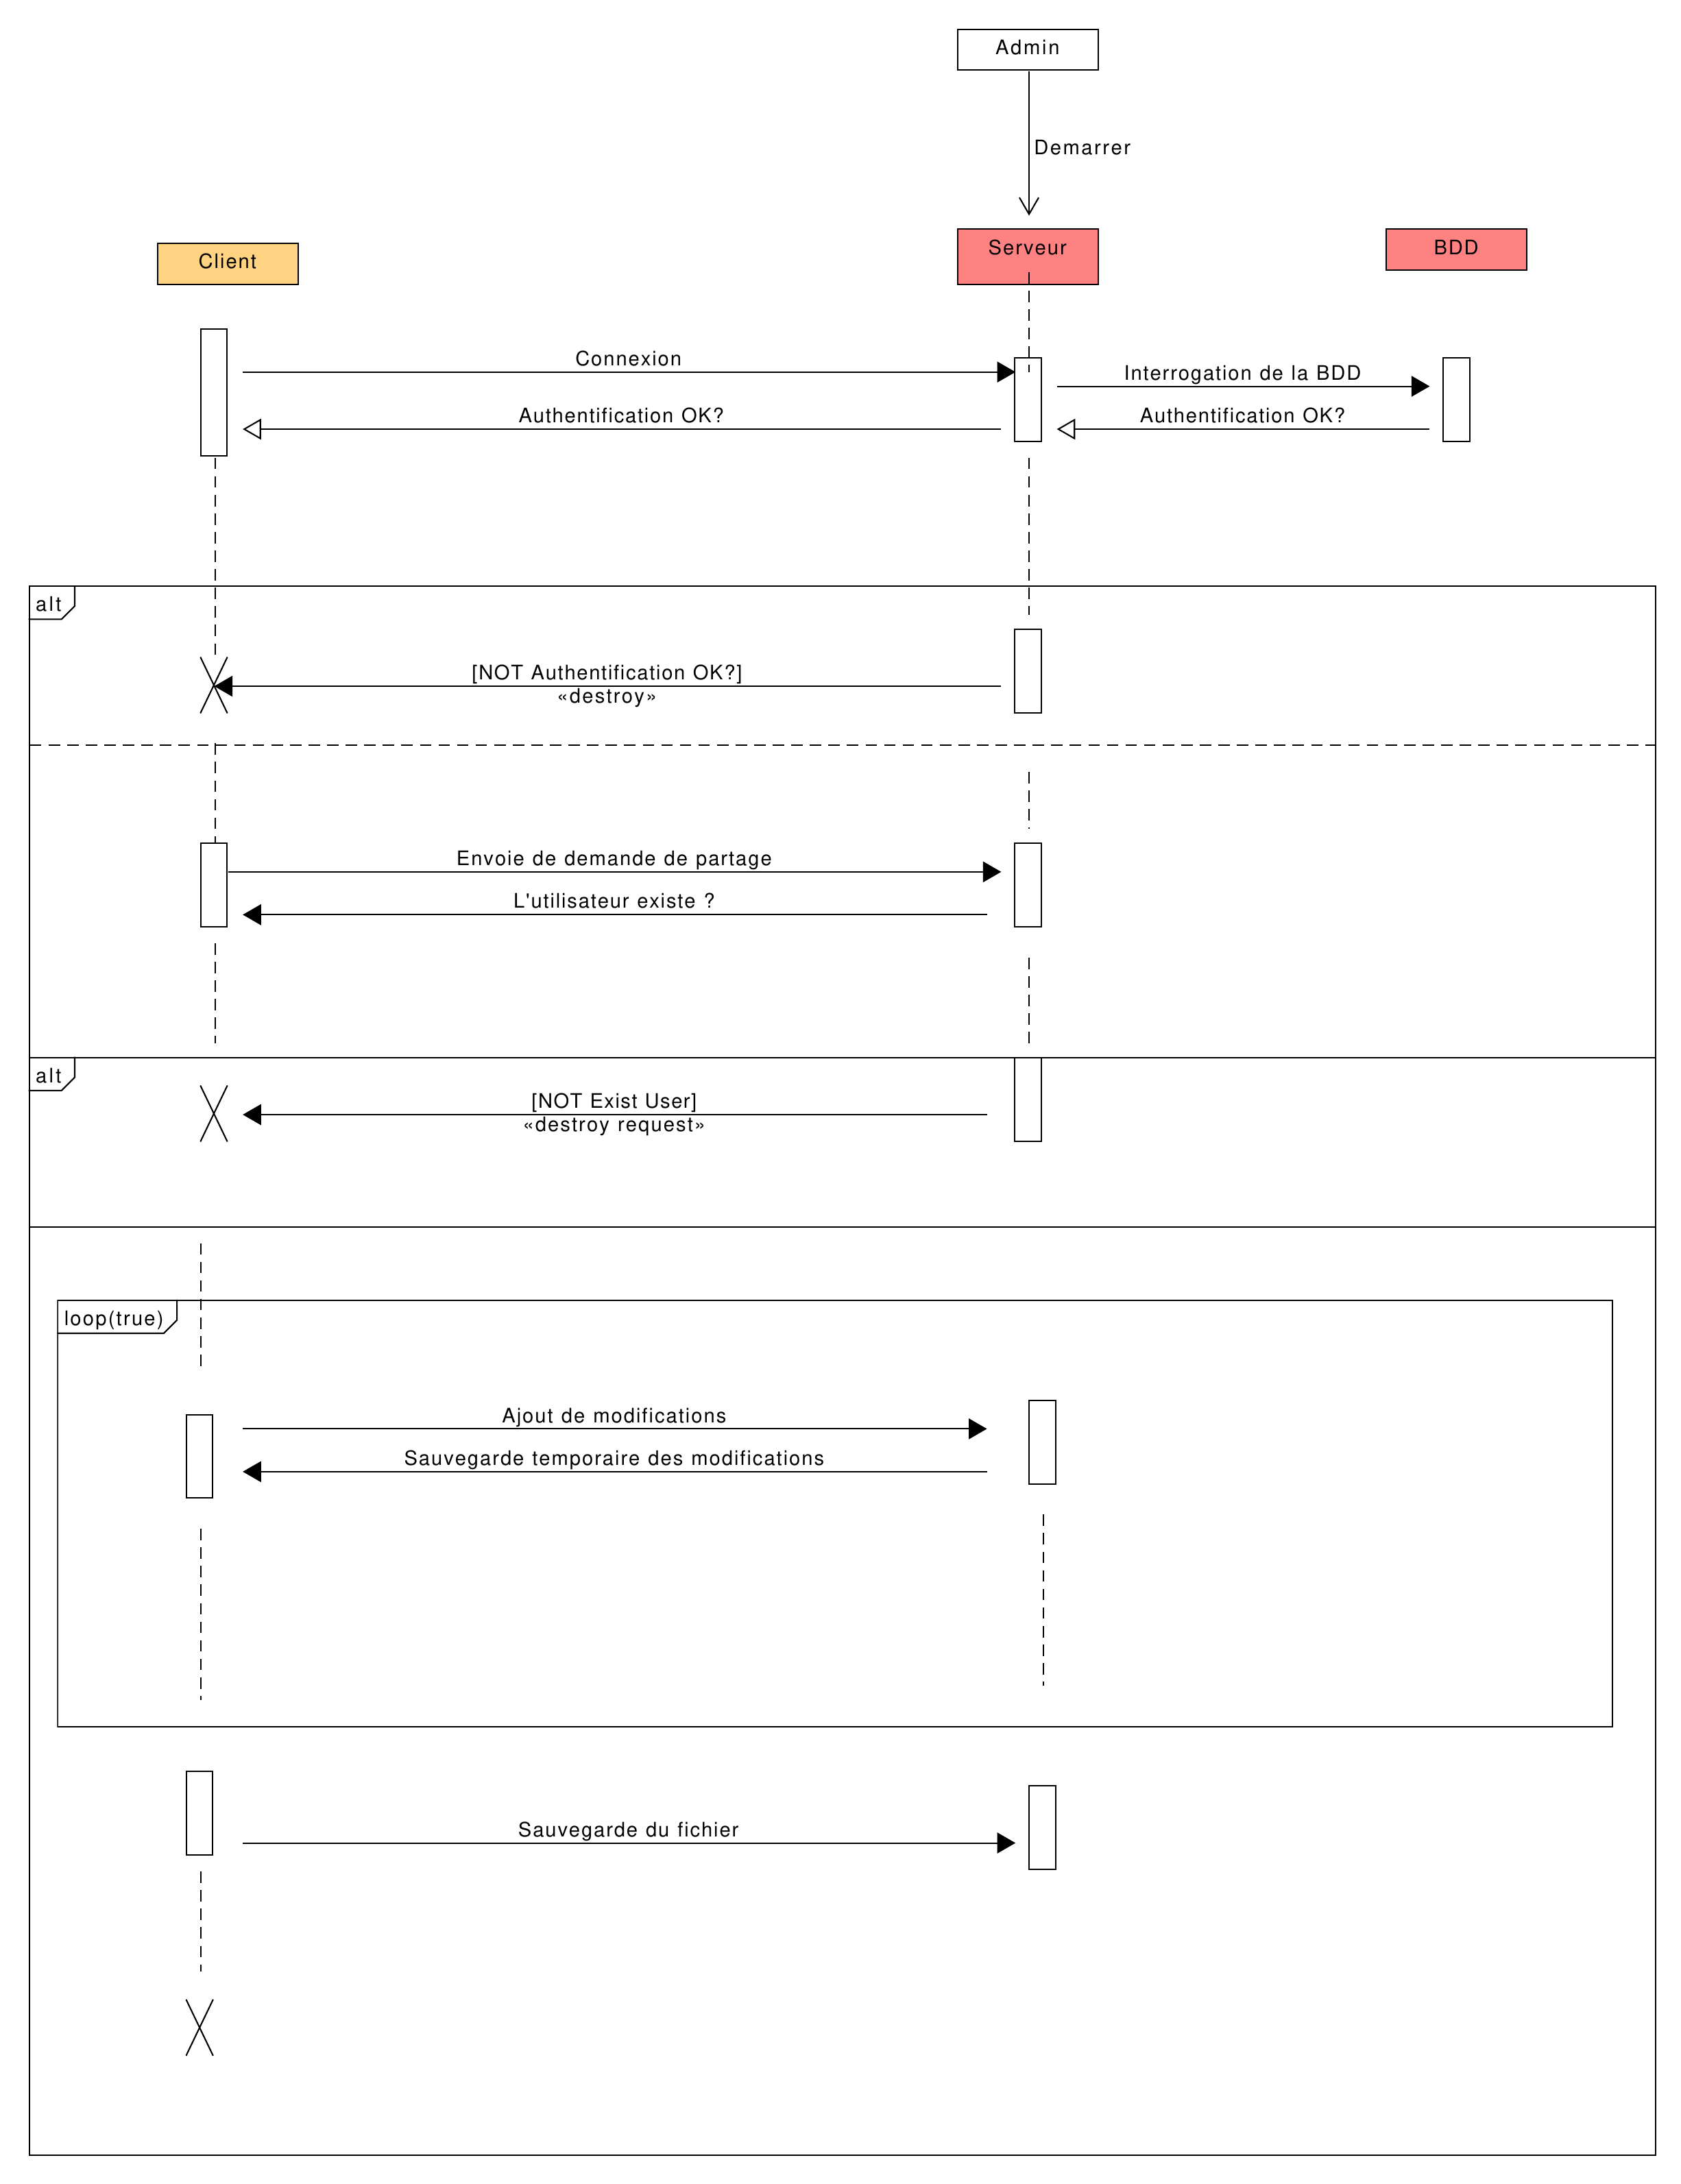
\includegraphics[scale=.13]{setup/diagramme_sequence_partage.png}
		
		\caption{Diagramme de séquence de partage}
		\vspace*{1em}
	\end{figure}
	
	\newpage
	
	\subsection{Diagramme de création}
	
	\begin{figure}[hb]
	\centering
	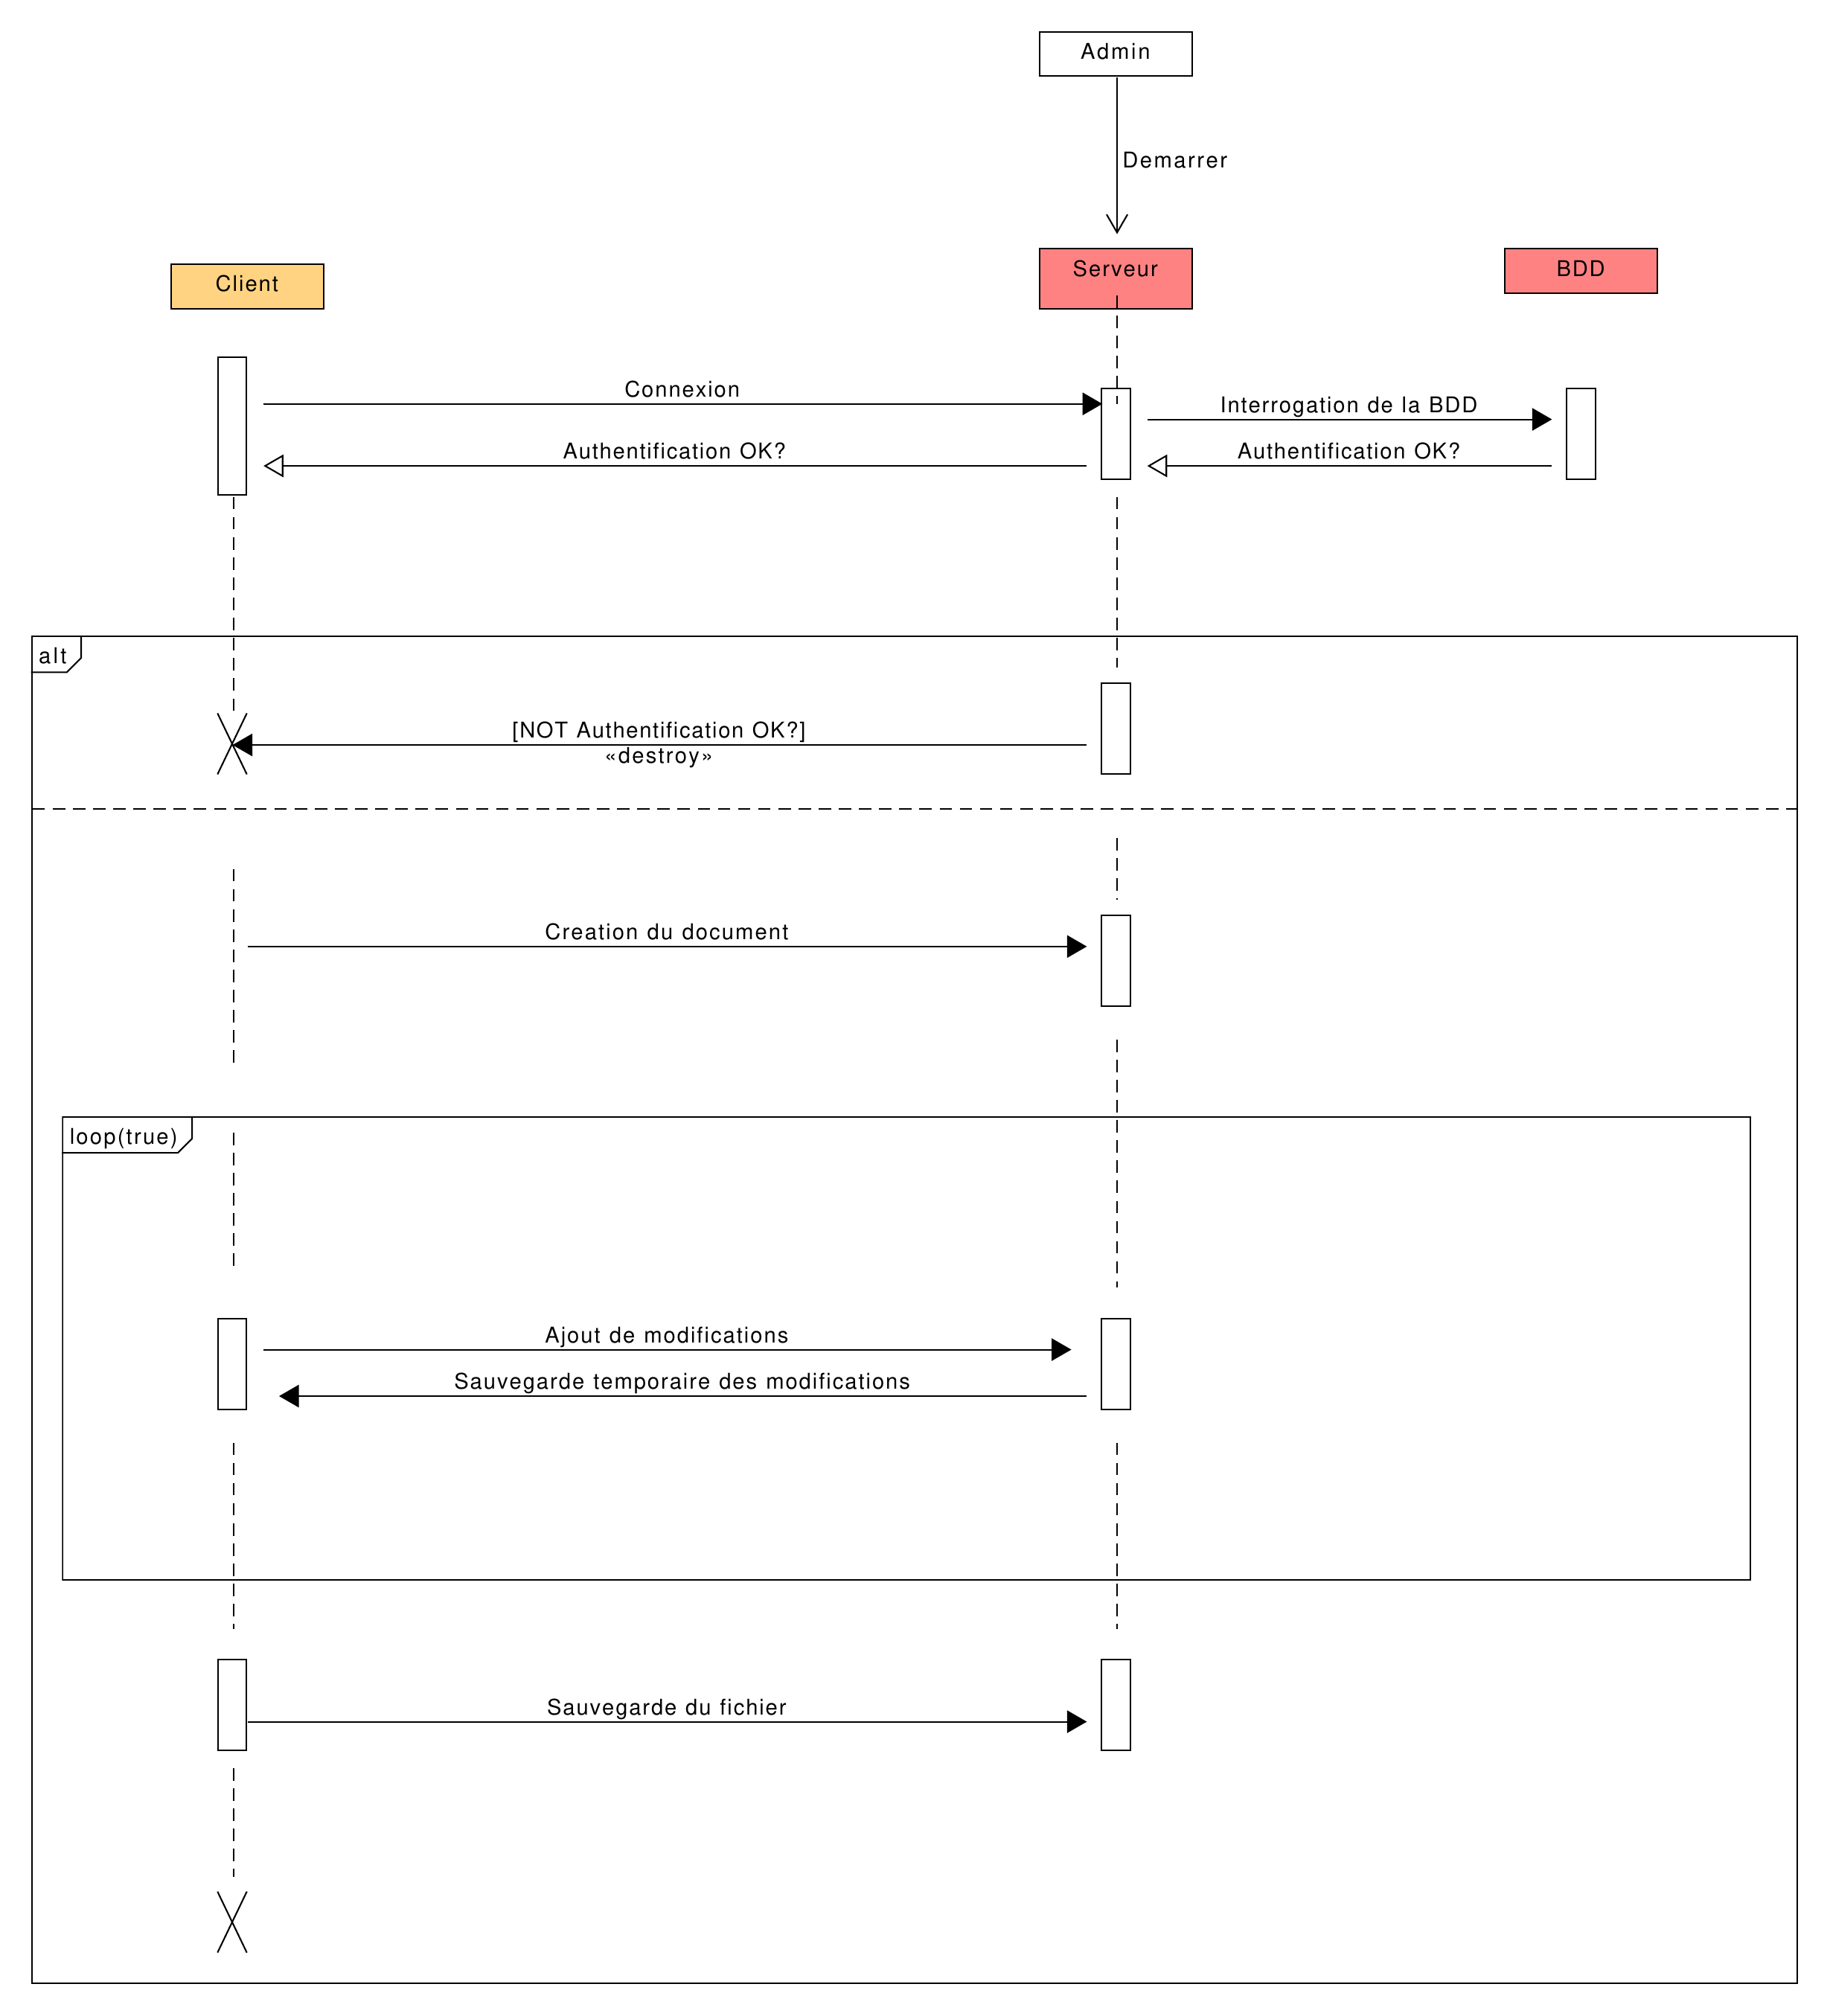
\includegraphics[scale=.32]{setup/diagramme_sequence_creation.png}
	
	\caption{Diagramme de séquence de création}
	\end{figure}
	
	\newpage
	
	\subsection{Diagramme de séquence de suppression}
	
	\begin{figure}[hb]
	\centering
	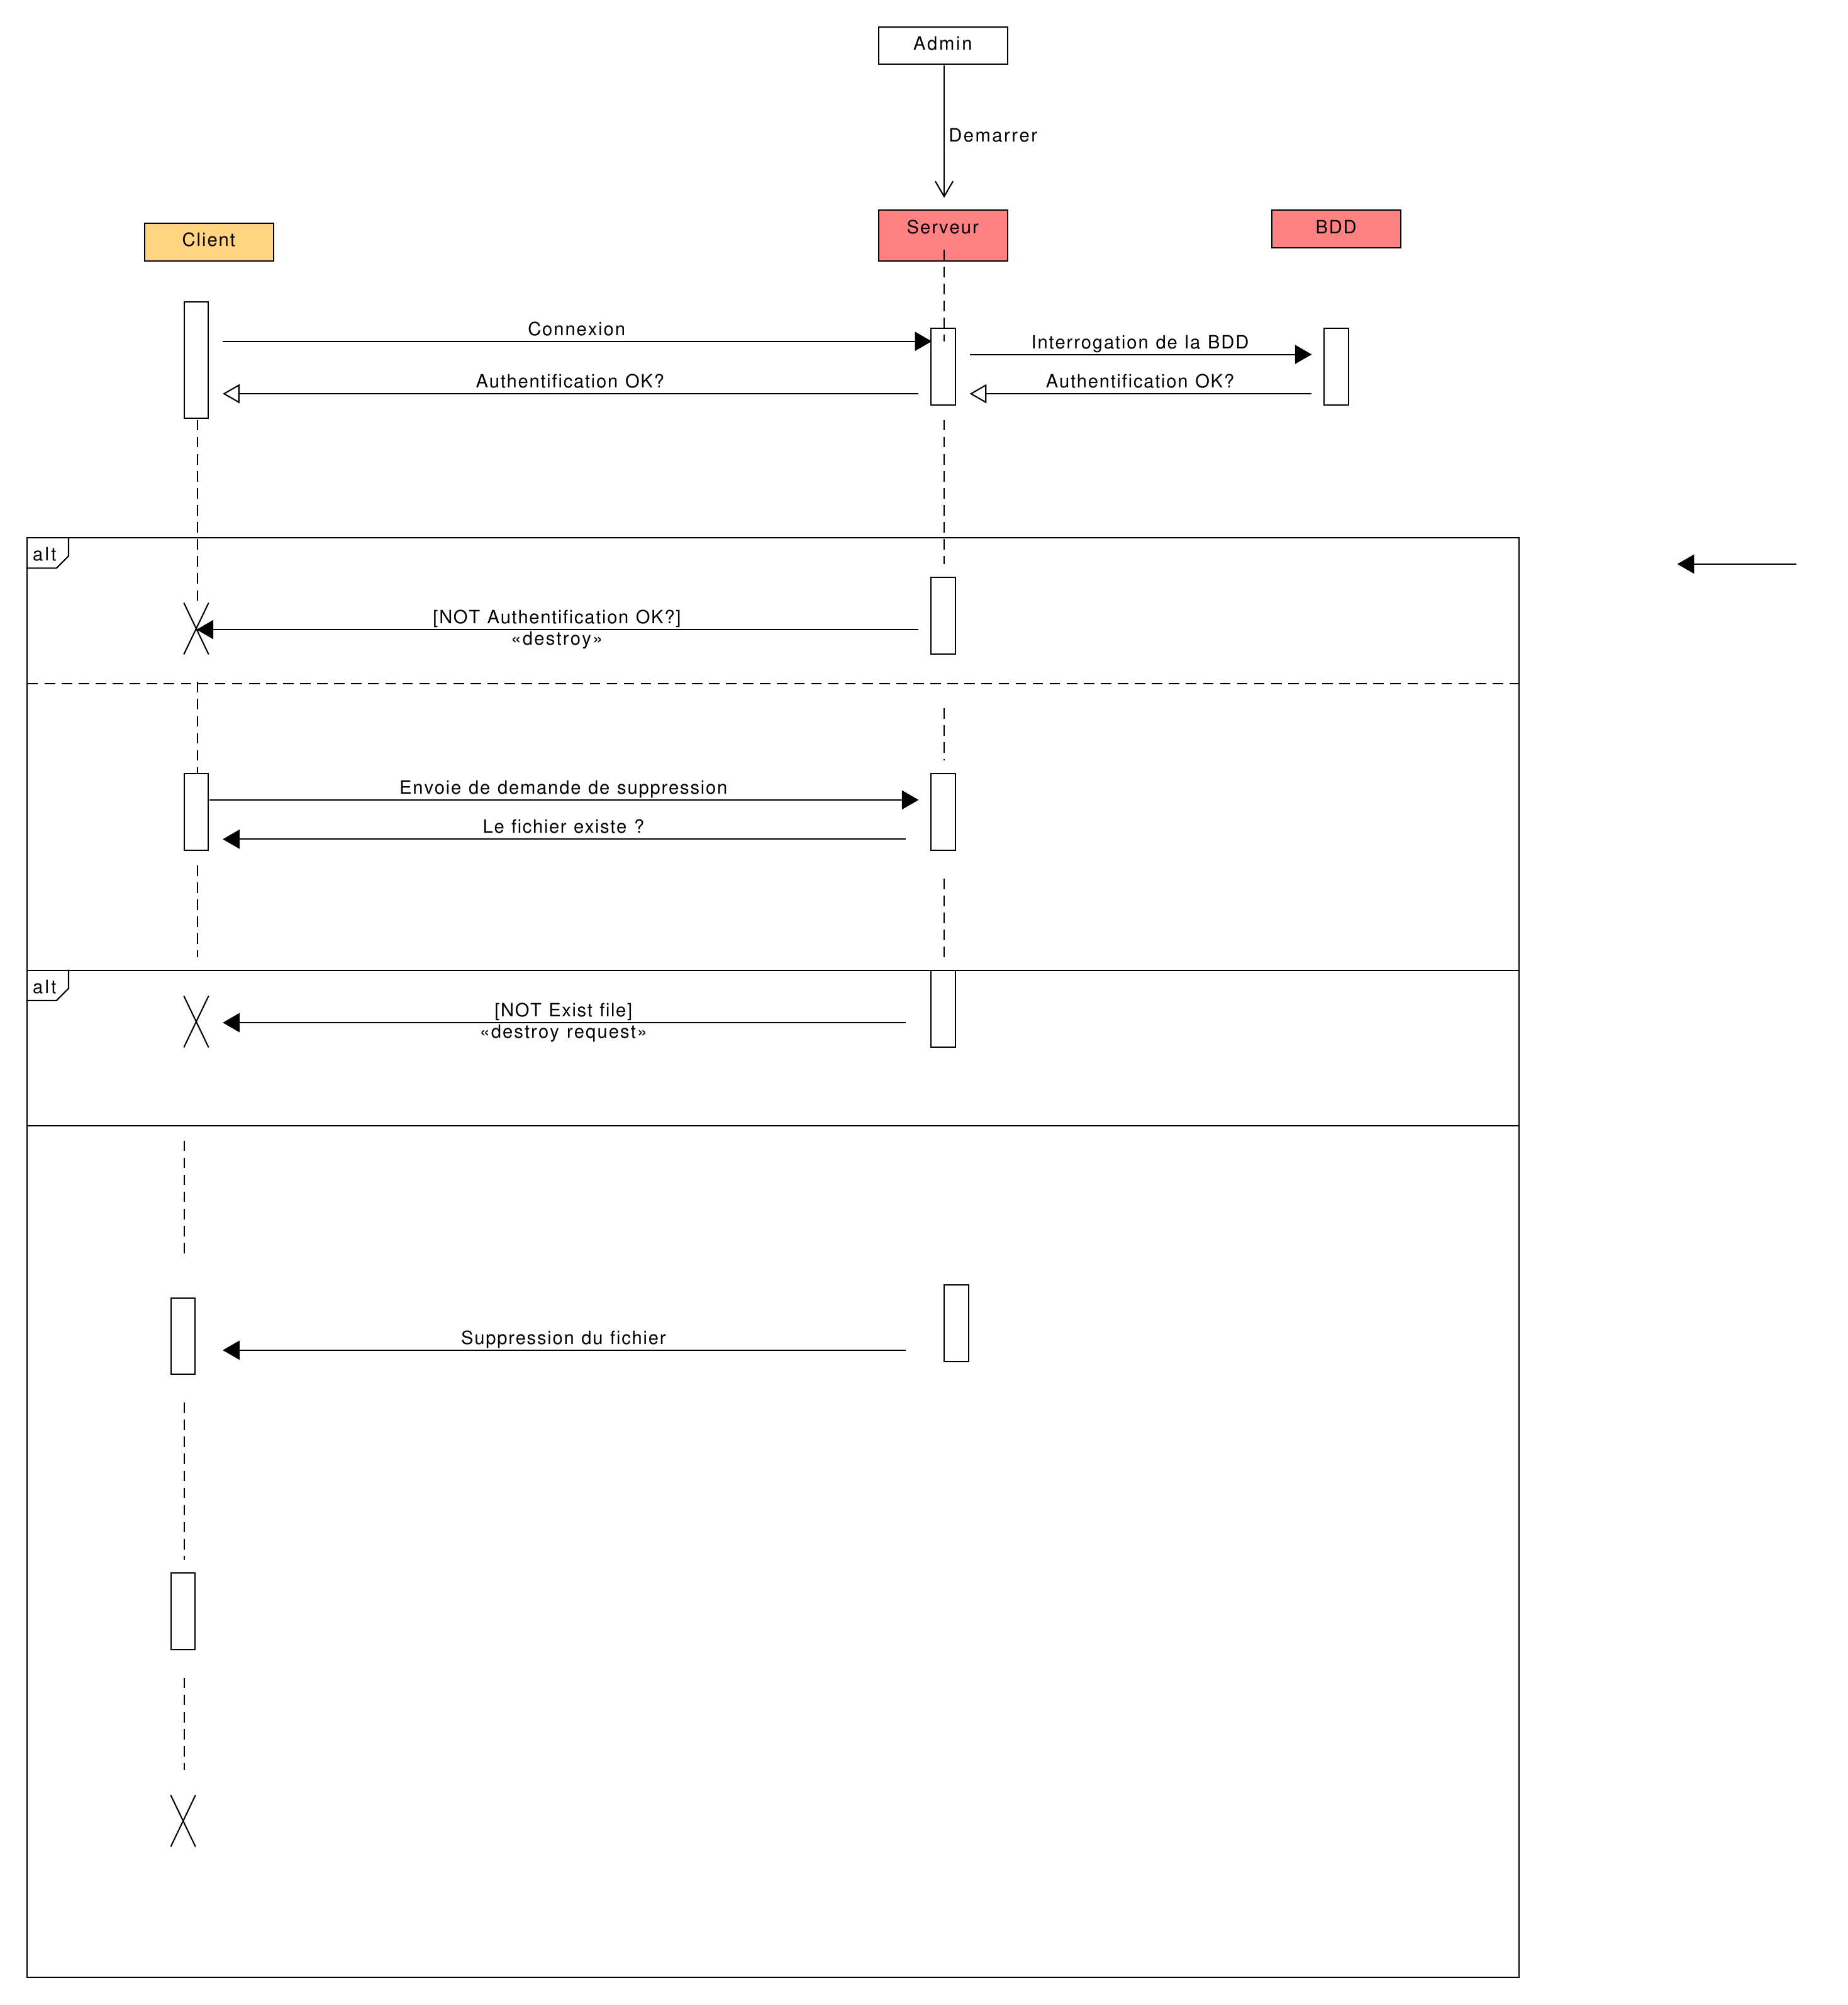
\includegraphics[scale=.3]{setup/diagramme_sequence_suppression.png}
	
	\caption{Diagramme de séquence pour le cas de la suppression d'un fichier}
	\end{figure}

	\newpage	
	
	\subsection{Modèle de l'interface pour une version initiale}
	
	\begin{figure}[hb]
	\centering
	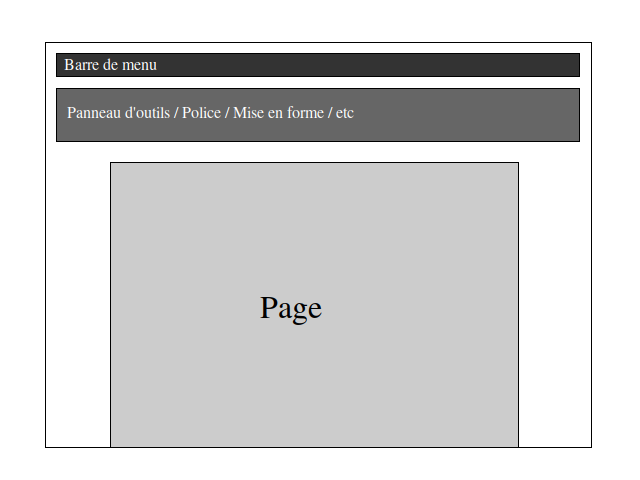
\includegraphics[scale=.6]{setup/modele_interface.png}
	
	\caption{Modèle de l'interface pour une version initiale}
	\end{figure}	
	
	\newpage
	
	\subsection{Modèle entité-assiocation de la base de données initiale}
	
	\begin{figure}[hb]
	\centering
	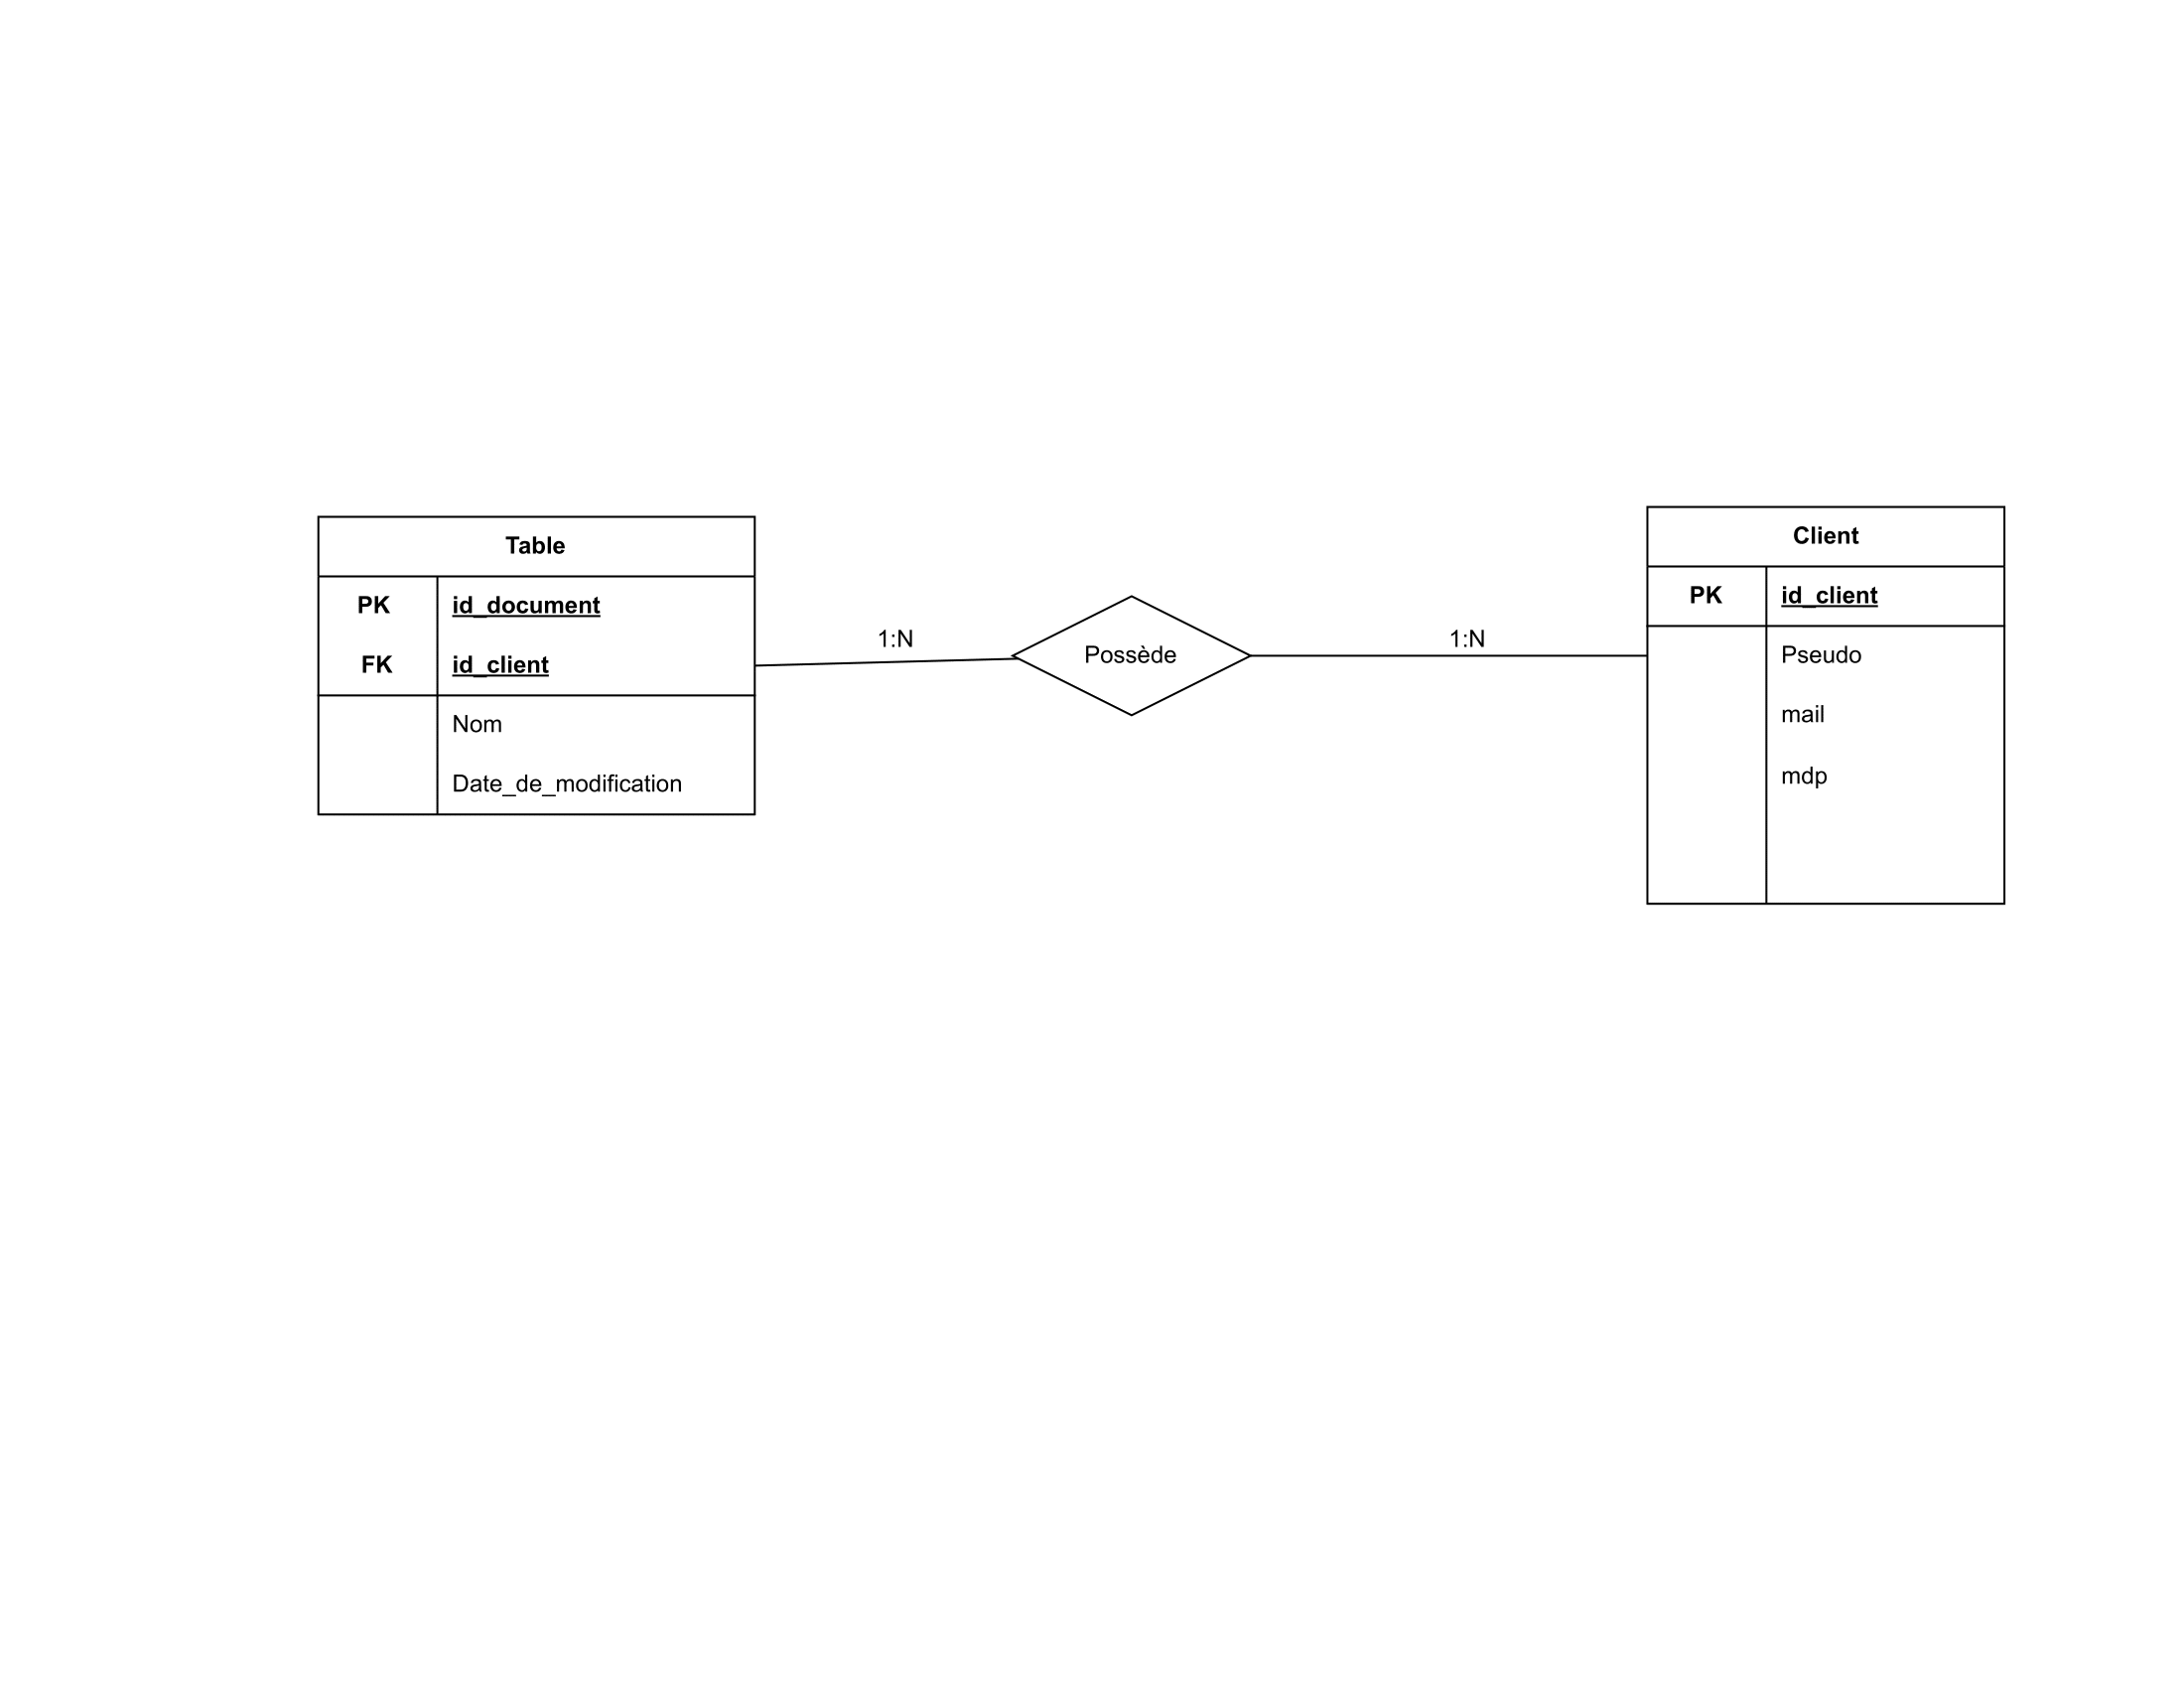
\includegraphics[scale=.5]{setup/modele_entite_association.png}
	
	\caption{Modèle entité-assiocation de la base de données initiale}
	\end{figure}
		
\end{document}